\chapter{Transactions}
	\section{Definition}
		\begin{itemize}
			\item Transaction resembles flow $($cash, goods, etc.$)$
			\item Transactions are the reason for business in the first place
			\item Application systems must support transaction programs!
			\item \color{red}"Transactions are the heart of economy"\color{black}
		\end{itemize}
			
	
	\section{Concept}
		\begin{itemize}
			\item A transaction is a process, that accesses and may updates data items
				\subitem databases 
				\subitem resource managers
			\item A transaction must see a consistent database at start
			\item During transaction, a database may enter a inconsistent state
			\item After the transaction is done, the Database must be consistent again
			\item There are 2 possible issues:
			\subitem Recovery $($ system crashes and similar $)$ 
			\subitem Concurrency Control $($ keeping the data consistent while multiple transactions are executed $)$
		\end{itemize}
	
	\newpage
	\section{Concurrent Executions}
%		\begin{figure}[h!]
%			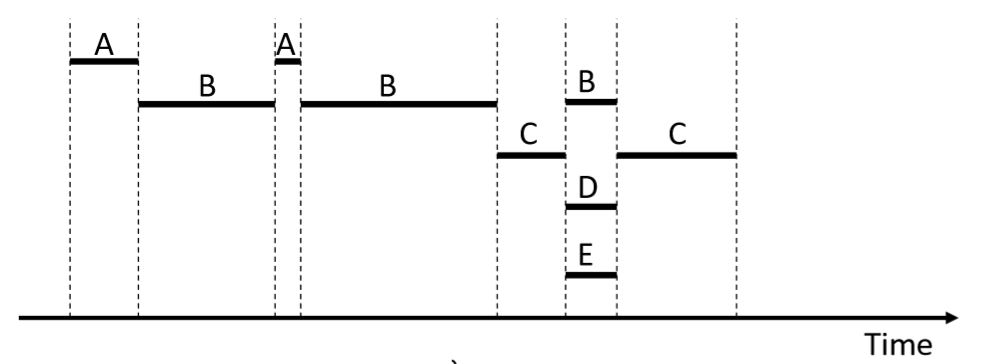
\includegraphics[scale=0.5]{res/Concurrent-Transactions.jpg}
%			\caption{Types of Concurrent Transactions}
%		\end{figure}
		\begin{itemize}
			\item A,B,C: Interleaved
			\item B,D,E: Simultaneous
			\item all: Parallel Transactions			
		\end{itemize}
	
	\section{Benefits of Concurrency}
		\begin{itemize}
			\item Higher Throughput
			\item More Utilization of the CPU = better value
			\item faster Response Time
		\end{itemize}
		
	\section{Possible Failures}
		\begin{itemize}
			\item System crash
			\item Transaktion Error
			\item Concurrency Control Enforcements $($Scheduler aborts$)$
			\item Disk Failure $($Data lost$)$
			\item Physikal Problems $($wrong Disk hooked up, Fire etc.$)$ 
		\end{itemize}
		
	
	\section{Transaction Processing}
		Transaction Processing is about:
		\begin{itemize}
			\item Maximum throughput
			\item Maximum utilization
			\item Maximum availability 
			\item Maximum scalability
			\item Minimum downtime
		\end{itemize}
	
	\section{ACID}
		\begin{itemize}
			\item Atomicity
				\subitem Transactions are fully reflected in the Resource Manager or are not reflected
			\item Consistency
				\subitem The Consistency of the resources is not harmed by any Transaction
			\item Isolation
				\subitem Transactions made at the same Time, don't need to know from each other to achieve correctnes
			\item Durability
				\subitem If a transaction is completed succesfully, all changes are permanent
		\end{itemize}
	
	\section{Transaction Operations}
	
		\subsection{BOT = Begin of Transaction}
		
			\subsubsection{Implicit BOT}
				
			\subsubsection{Explicit BOT}
		
		\subsection{EOT = End of Transaction}
		
			\subsubsection{Implicit EOT}
		
			\subsubsection{Explicit EOT}
		
		\subsection{COMMIT}
			Request to make all changes permanent
		
		\subsection{ABORT/Roll back}
			All changes must be reverted
		
	\section{Example in RL}
		\begin{figure}[h!]
			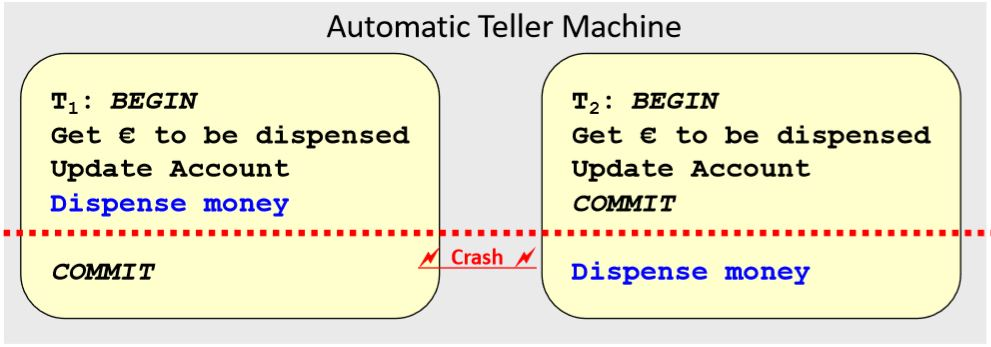
\includegraphics[scale=0.5]{res/real-life-transaction.jpg}
			\caption{Real World Actions In Transactions}
		\end{figure}
	
	\section{Transaction States}
		\begin{itemize}
			\item active
				\subitem  the initial state; the transaction stays in this state while it is executing 
			\item done
				\subitem all statements have been executed
			\item failed 
				\subitem n
			\item aborted normal execution can no longer be achieved
			\item commited
				\subitem after successful completion
			\item aborted
				\subitem transaction was aborted and all changes are reverted
		\end{itemize}
			
		\begin{figure}[h!]
			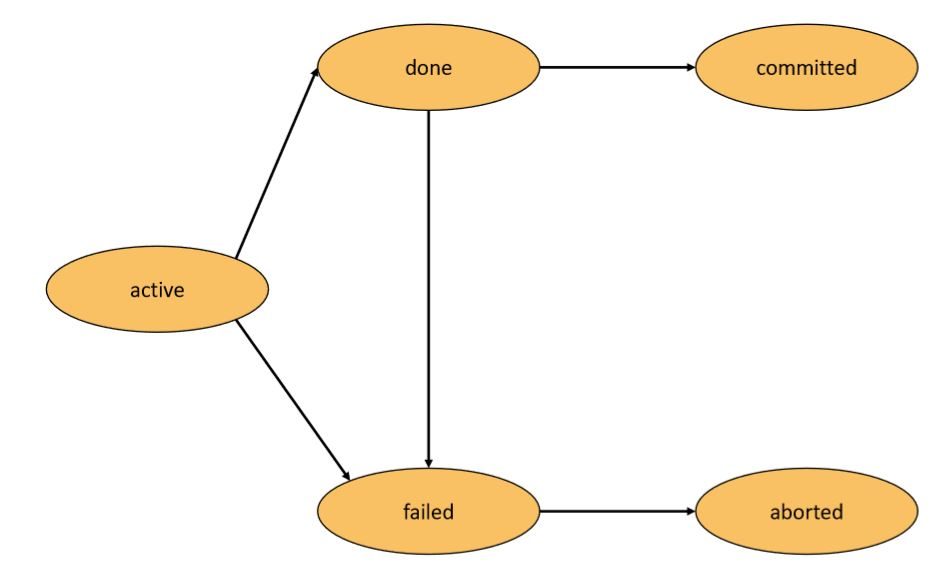
\includegraphics[scale=0.5]{res/state-diagram-transaction.jpg}
			\caption{Transaction State Diagram}
		\end{figure}
	
	\section{Serializability}
		
		
		
		
		
		
			
		